\section{UserCSP Design}
\label{sec:design}

The goal of our approach, \codename, is to help web site
administrators and users of a website to write comprehensive CSP rules
for the website.

\begin{figure}[h!]
\center
  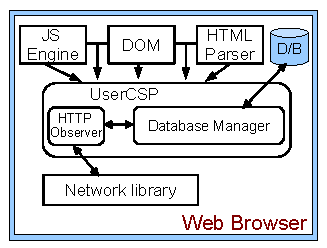
\includegraphics{userCSP_Arch}
\caption{\codename Architecture}
\label{fig:userCSP-Arch}
\end{figure}

Figure~\ref{fig:userCSP-Arch} illustrates the architecture of
\codename. To enforce user specified content sencurity policy as well
as to infer CSP policy for a website, \Codename monitors web browsers
internal events including HTML parsing, HTTP requests, XHR, etc., and
analyzes the type of content loaded by a web page and source of that
content. Database manager component of the \codename is responsible
for storing user specified CSP policies for websites into local
database and retrieves the corresponding CSP policy for the website
when user loads the website.

When users visits a website, \Codename performs one of the following
actions:

\begin{itemize}

\item If website has defined CSP policy but user doesn't specify a CSP
  policy for the website then \codename doesn't interfere with the
  website defined CSP policy. However, it allows user to amend
  website CSP policy if user wants it.

\item If user has specified a CSP policy for a website but the website
  administrators didn't set a CSP policy for their website then user
  specified CSP policy will be enforced by the \codename.
 
\item If user specified CSP exists as well as website defined CSP
  exits then users have a choice either to apply their own policy or
  adopt website defined policy. Moreover, users can also select strict or
  loose set of CSP policy by combining their own policy with website
  defined policy. For example, if a website sets ``script-src
  www.example.com;'' and user specified ``script-src www.example.com
  www.abc.com;'' then strict set will set ``script-src
  www.example.com;'' whereas loose set will set ``script-src
  www.example.com www.abc.com;''.

\item if neither user nor website administrators specified a CSP
  policy for the website then \codename doesn't interfere with the
  content loading of the website. 

\item To allow automatic infer of a CSP policy for websites, \codename
  monitors contents loaded by web pages and recommends a CSP policy
  based on the types of contents and sources of that content. It also
  monitors the resources dynamically added to the web page by
  JavaScript.

\end{itemize}
